\documentclass[conference]{IEEEtran}
\usepackage{cite}
\usepackage{amsmath,amssymb}
\usepackage{graphicx}
\usepackage{booktabs}
\usepackage{array}
\usepackage{url}
\usepackage{balance}
\graphicspath{{figures/}}

\title{Design and Resource Evaluation of a Hybrid Quantum--Classical Chess Prototype Using Grover-Based Move-Index Amplification}

\author{\IEEEauthorblockN{Team 1}
\IEEEauthorblockA{Amrita Vishwa Vidyapeetham\\
Section A}}

\begin{document}
\maketitle

\begin{abstract}
This paper presents a hybrid quantum--classical chess prototype and evaluates its circuit resources and simulator runtime. The system combines classical legal-move generation and heuristic ranking with Grover-based amplification over indices of selected candidate moves. It also includes a small-board circuit that processes a supplied move and a register-level demonstration of coordinate and square-status encoding. A benchmark on four seeded 3$\times$3 positions reports mean times of 1.19 ms for depth-3 classical minimax, 95.81 ms for the supplied-move circuit path, and 71.74 ms for the hybrid path using Qiskit Aer. These paths perform different workloads and are measured on a classical simulator. Legal-move generation and heuristic target selection remain classical, and the small-board transition circuit does not implement a complete reversible board update. The measurements characterize this prototype and do not establish quantum speedup or improved playing strength.
\end{abstract}

\begin{IEEEkeywords}
chess engine, Grover search, hybrid quantum-classical computing, minimax, Qiskit Aer, simulator evaluation
\end{IEEEkeywords}

\section{Introduction}
\subsection{Motivation and Problem Setting}
Chess move selection combines legal-move generation, position evaluation, and search over possible continuations. These tasks are interdependent: a legal move can be strategically weak, and the value of a move can depend on a sequence of later replies. Shannon's early analysis of computer chess established search and position evaluation as central computational concerns \cite{shannon1950}. Classical programs address this structure with game-tree methods such as minimax, often combined with alpha--beta pruning to avoid exploring branches that cannot affect the selected result \cite{knuth1975}.

Quantum computing offers algorithms for specific search and sampling problems, but its relevance to chess depends on how the chess computation is represented. Grover's algorithm and the more general amplitude-amplification framework increase the probability of measuring a candidate marked by a Boolean predicate. For a search space of $N$ candidates containing $M$ marked candidates, the ideal query complexity is on the order of $\sqrt{N/M}$ oracle applications \cite{grover1996,boyer1998,brassard2002}. This is a query-complexity result; it does not by itself include the cost of preparing candidates, constructing the oracle, or implementing a reversible evaluation of each candidate.

Applying this primitive to chess therefore requires a precise account of what the oracle evaluates. If legality and move quality are computed classically before the circuit is built, the circuit searches a classically prepared set of marked indices. It does not search the full game tree or evaluate chess positions in superposition. A system that makes those stronger claims would require a reversible board representation, reversible move and legality computation, and uncomputation of intermediate data. These requirements motivate evaluating both the implemented circuit and the boundary between its quantum and classical stages.

\subsection{Quantum Search and Chess Computation}
The distinction between quantum search and quantum chess is important. In a quantum-chess rule variant, the game itself incorporates quantum behavior such as superposition, entanglement, or measurement \cite{cantwell2019}. The project examined here retains classical chess rules and uses quantum circuits as computational components. It therefore investigates a hybrid implementation strategy rather than defining a new quantum chess ruleset.

Prior work has studied quantum algorithms for evaluating minimax and NAND trees, connecting quantum computation more directly to game-tree evaluation \cite{cleve2008,farhi2008}. Those algorithms address structured tree-evaluation problems under specific oracle and query models. They are distinct from applying Grover search to a list of move indices that have already been generated and scored by classical code. Keeping these algorithmic settings separate is necessary when interpreting the prototype's results.

\subsection{Project Scope and System Overview}
This paper examines a prototype with three related implementations. The 8$\times$8 hybrid path uses classical code to generate legal moves and assign heuristic scores. The highest-scoring move indices are supplied to a Grover-based circuit, which amplifies their measurement probability. Classical code decodes the measured index and maps it back to the move list. The quantum stage operates on candidate indices; it does not compute legal moves or their heuristic scores.

The 3$\times$3 implementation provides a small-scale comparison among three paths: depth-3 classical minimax, a circuit that processes a supplied move, and a hybrid selector that scores candidate moves classically before applying Grover search to their indices. The supplied-move circuit demonstrates register construction and gate operations, but it does not independently choose a move or perform a complete quantum board update. The 2$\times$2 implementation provides a smaller gate-level example for tracing coordinate and square-status registers. These implementations share a project context, but their functions and workloads differ.

Across all three paths, the classical board state remains authoritative. The hybrid circuit returns a candidate index for classical decoding and subsequent game-state handling. The small-board coordinate and status circuits are separate demonstrations; their measurement results do not feed the hybrid move-index selector. This separation makes the system data flow inspectable and defines the scope of the claims made in this paper.

\subsection{Research Questions and Design Objectives}
The study is guided by three practical questions. First, how can a classical chess application be connected to a quantum search circuit while keeping the input, oracle, measurement, and output stages explicit? Second, what circuit-resource and simulator-runtime measurements result from the implemented classical, circuit, and hybrid paths on the available small-board benchmark? Third, which limitations in the present encoding and oracle boundary must be addressed before the system could support end-to-end quantum move evaluation?

These questions lead to four design objectives: document the data flow between classical and quantum components; distinguish the move-index search from the supplied-move circuit; report simulator measurements with their workload definitions; and identify the algorithmic and implementation work needed for a more complete reversible chess computation. The paper treats these as engineering and evaluation objectives. It does not assume that using a quantum circuit produces an advantage for this workload.

\subsection{Contributions}
The paper makes the following contributions:
\begin{itemize}
  \item It documents a multi-scale prototype comprising an 8$\times$8 hybrid move-index search, a 3$\times$3 comparison of classical and circuit paths, and a 2$\times$2 register-level demonstration.
  \item It describes the boundary between classical legal-move generation and heuristic ranking, and the Grover circuit that amplifies indices selected by that classical stage.
  \item It reports simulator measurements from four seeded 3$\times$3 positions, including runtime and circuit-resource results, with the measured workloads identified explicitly.
  \item It analyzes the prototype's limits, including the absence of a reversible chess-evaluation oracle and a complete quantum board-state transition in the small-board circuit.
\end{itemize}

\subsection{Evaluation Context}
The measured 3$\times$3 comparison includes depth-3 classical minimax, the supplied-move circuit, and the hybrid path. The reported mean times are 1.19 ms, 95.81 ms, and 71.74 ms, respectively. These values describe four seeded Qiskit Aer simulator runs \cite{aer2026} and workloads with different responsibilities: minimax selects a move by searching a shallow game tree, the supplied-move circuit processes a provided move, and the hybrid path generates and scores candidates before simulating Grover search.

The timing values should therefore be read as implementation measurements, not as a direct performance ranking of equivalent algorithms. In particular, the hybrid circuit's target indices are prepared using classical scoring, and the circuit runs on a classical simulator. The results do not demonstrate quantum speedup, improved playing strength, or performance on quantum hardware. They make the current system's runtime and circuit-resource costs visible and provide a baseline for more complete implementations.

\subsection{Organization of the Paper}
The remainder of the paper reviews related classical and quantum approaches, identifies the gap between those algorithms and the prototype's implementation, and explains the motivation and contributions. It then presents the system architecture, circuit encoding, and benchmark methodology, followed by measured results and their interpretation. The conclusion summarizes the findings and outlines work needed for reversible move evaluation and more rigorous end-to-end experiments.

\section{Related Work}
Shannon's early formulation of computer chess identifies move search and position evaluation as core engineering problems \cite{shannon1950}. Knuth and Moore analyze alpha--beta pruning as a method for reducing the game tree explored by minimax \cite{knuth1975}; the project uses this classical family for its depth-limited baseline. These methods search continuations in a game tree, whereas Grover search locates marked elements in a finite search space. They solve related selection tasks but are not interchangeable algorithms.

Grover introduced amplitude amplification for unstructured search, and later analyses addressed multiple marked items and iteration counts \cite{grover1996,boyer1998,brassard2002}. Quantum algorithms for evaluating NAND and minimax trees address game-tree evaluation more directly, but rely on different models and assumptions from a small Grover index circuit \cite{farhi2008,cleve2008}. Cantwell's quantum-chess work defines a chess variant whose rules use quantum behavior; it differs from this project's classical chess rules plus quantum search and circuit demonstrations \cite{cantwell2019}. Preskill discusses the practical constraints of noisy intermediate-scale quantum devices \cite{preskill2018}. LaRose surveys gate-level software platforms, and the Qiskit Aer documentation describes the simulator used here \cite{larose2019,aer2026}. Standard circuit notation and state-vector concepts follow Nielsen and Chuang \cite{nielsen2010}.

\section{Literature Gaps Identified}
The literature reviewed here supplies classical chess-search methods, quantum unstructured search, and quantum game-tree algorithms, but these do not provide a ready-made, end-to-end reversible oracle for the project's chess move representation. In particular, legal-move generation, reversible scoring of chess positions, and complete board-state updates must be designed before Grover can search chess moves coherently. The distinction between quantum chess as a rule variant and quantum search applied to classical chess move lists also needs to be explicit. Finally, simulator resource counts alone cannot establish practical speedup: workload equivalence, oracle cost, noise, measurement, and move quality must be evaluated. These gaps motivate an implementation study focused on transparent data flow and bounded claims rather than an advantage claim.

\section{Why Quantum and Project Contributions}
Quantum search is relevant as a way to explore whether a list of move candidates can be represented by indices, marked by a predicate, and sampled after amplitude amplification. The project's present oracle receives target indices selected by a classical heuristic, so this is an educational integration experiment rather than a quantum replacement for minimax. Keeping the distinction explicit helps identify the algorithmic work required for a meaningful quantum chess-search result.

The project makes the following three contributions:
\begin{itemize}
  \item It implements and documents three board-scale demonstrations: 2$\times$2 gate tracing, 3$\times$3 classical and circuit comparison, and 8$\times$8 hybrid move-index search.
  \item It connects classical legal-move generation and heuristic ranking to a Qiskit Grover circuit, and separately exposes coordinate/status encoding and controlled-gate behavior in the small-board prototype.
  \item It reports reproducible simulator timing and circuit-resource measurements for four seeded 3$\times$3 positions, together with limitations that prevent those measurements from supporting quantum-speedup or playing-strength claims.
\end{itemize}

\section{Methodology}
\subsection{Systems and Data Flow}
\textbf{8$\times$8 hybrid system:} the classical move generator creates legal moves from the board. A heuristic assigns each move a score using capture value, pawn advancement, and center preference. Python collects all indices tied for the highest score. The Grover circuit prepares a uniform superposition over a padded binary index space, phase-marks those indices, applies a diffuser, and measures an index. Classical code decodes the result, validates it against the move list, and applies the move to the classical game state. A depth-3 minimax fallback is available when the quantum path cannot return a move. The circuit's input list and marked set are prepared classically.

\textbf{3$\times$3 systems:} the classical baseline selects a move using depth-3 minimax with alpha--beta pruning and heuristic move ordering. The pure-circuit route receives a predetermined legal move, loads its coordinates and square statuses into a 23-qubit circuit, runs limited direction/status logic, and measures the registers. It demonstrates circuit construction and measurement; it does not autonomously choose the move or update the board. The hybrid comparison generates legal moves and scores them classically, then simulates Grover over the top-scoring move indices. The normal 3$\times$3 game route uses classical minimax for AI selection; the hybrid comparison is a separate evaluation path.

\textbf{2$\times$2 system:} a single Black Pawn at $(0,0)$ is used to explain how source and target coordinates, status lookups, and controlled gates are represented. On this board, a candidate move such as $(0,0)\rightarrow(1,0)$ is encoded in the small-board registers. This example is a gate-level demonstration, not a complete implementation of pawn legality or a quantum board transition. Grover's move-index circuit is a separate circuit and is used only when the candidate-search path has a nontrivial set of options.

\begin{figure*}[t]
\centering
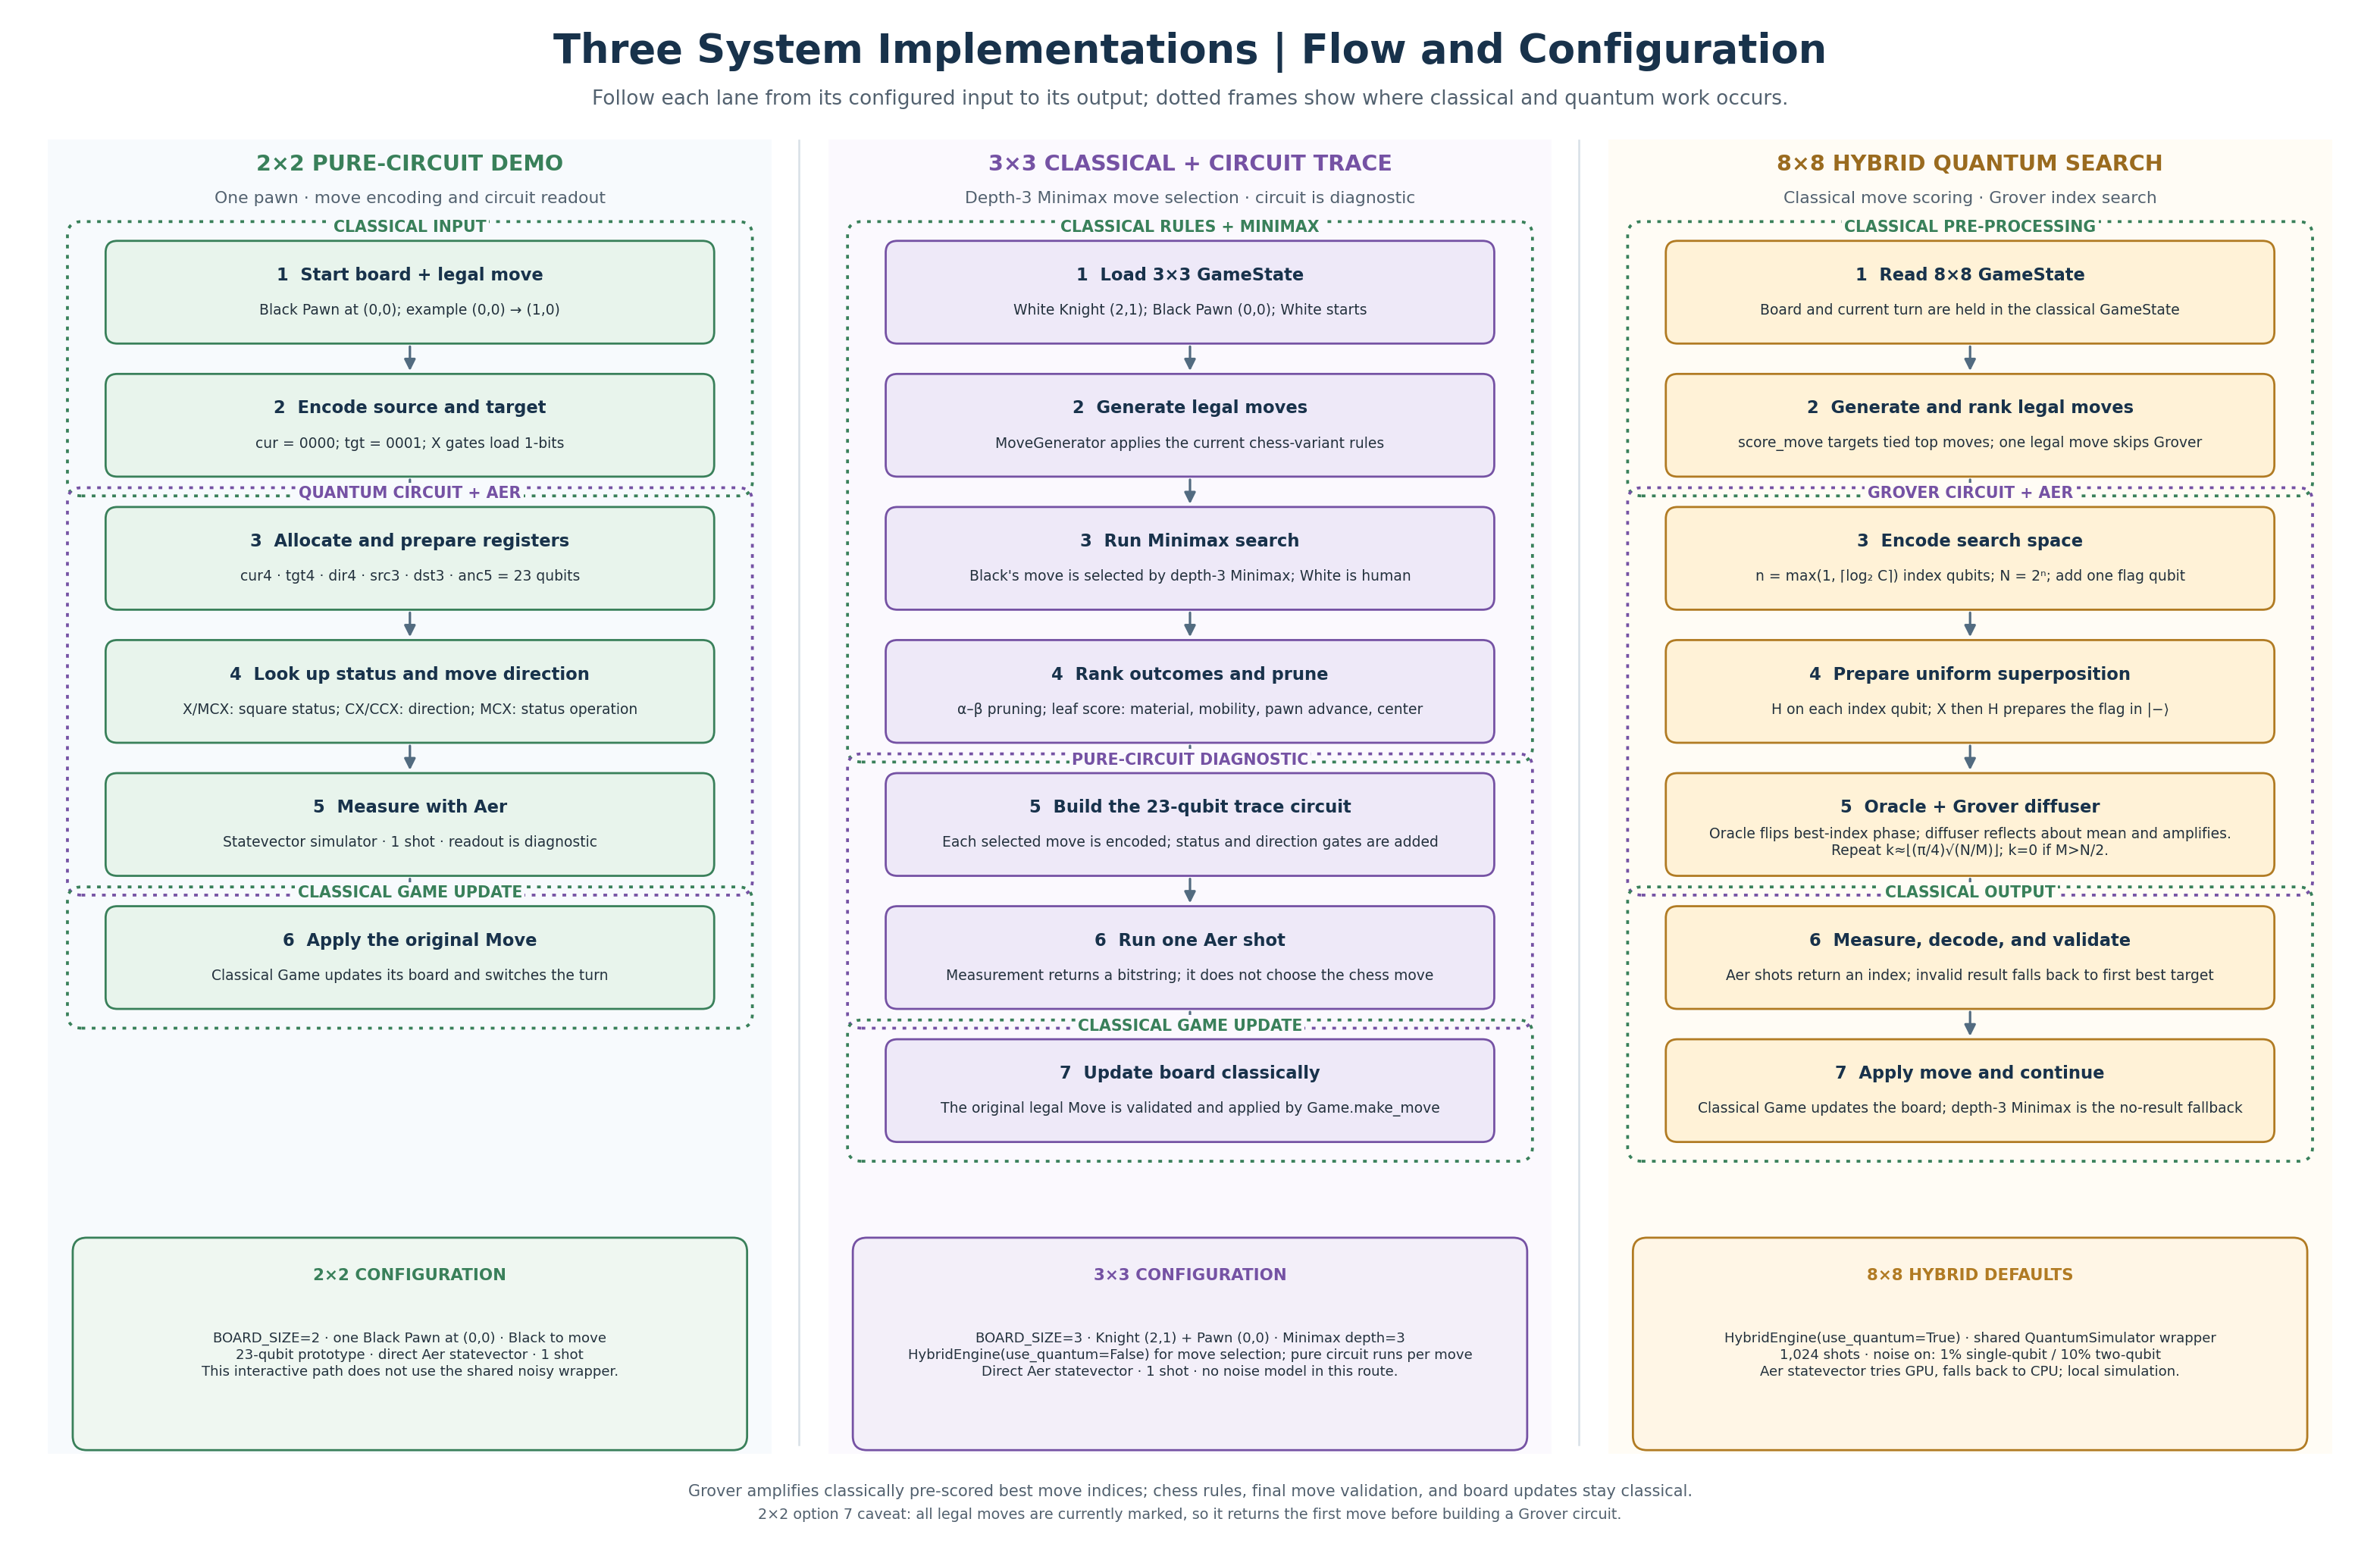
\includegraphics[width=0.96\textwidth]{08_detailed_system_implementation_flows.png}
\caption{The three implementation flows and their classical and quantum stages. Classical code owns legal-move generation, evaluation, and board updates; the hybrid circuit searches marked candidate indices.}
\label{fig:architecture}
\end{figure*}

\subsection{Quantum Encoding and Grover Circuit}
For the small-board circuit, a coordinate uses two bits for column and two for row. A 2$\times$2 source at $(0,0)$ maps to $0000$; target $(1,0)$ maps to $0001$ under the project's logical column-then-row convention. The circuit allocates source and target coordinates (4 qubits each), direction workspace (4), source and destination status (3 each), and ancilla workspace (5), for 23 qubits total. Status values include empty $000$ and Black Pawn $001$. The builder uses $X$ gates to prepare one-bits and to convert zero-controls into positive controls, $CX$ and $CCX$ for limited direction logic, and multi-controlled $X$ gates for coordinate-conditioned status lookups and attempted status operations. The actual board transition remains classical.

For Grover, $n=\lceil\log_2 C\rceil$ index qubits represent $C$ candidates in a padded space of $2^n$. Hadamard gates prepare the uniform state $|s\rangle$. The flag is prepared in $|{-}\rangle$; the oracle's multi-controlled $X$ then produces phase kickback, multiplying marked-index amplitudes by $-1$. The diffuser $D=2|s\rangle\langle s|-I$ reflects amplitudes about their mean. The oracle and diffuser are repeated for an iteration count estimated from the search-space and target counts. Measurement returns a bit string that classical code decodes to a move-list index. The oracle does not compute chess legality or heuristic scores coherently: those are computed before circuit construction.

\subsection{Benchmark Design and Configuration}
The comparison uses four unique 3$\times$3 positions generated deterministically from authored piece layouts and seeded legal random walks (seed 20261013). There is no external training dataset and no learned model, so train/test splitting is not applicable. The classical model is depth-3 minimax; the pure-circuit input is the first legal move in each position and uses one shot; the hybrid path scores the candidate list classically and runs Grover with 2048 shots. Both quantum paths use Qiskit Aer on CPU with the matrix-product-state method and noise disabled. Simulator initialization is excluded from per-position timing. These settings are specific to this comparison; the shared application wrapper defaults to 1024 shots and an illustrative depolarizing noise model.

The reported metrics are mean elapsed time per position; mean additional process resident memory above the pre-step baseline, sampled every 2 ms; average legal-move count; qubit count; circuit gate count; and circuit depth. Memory sampling is approximate and may miss short peaks. Circuit metrics are not applicable to the classical selector. Timing covers move selection for classical minimax, circuit construction plus simulation for the pure route, and candidate generation/scoring plus Grover-circuit construction, transpilation, and simulation for the hybrid route. This is a small engineering benchmark, not a statistically powered or hardware comparison.

\section{Results and Analysis}
Table~\ref{tab:results} reports the benchmark means. Fig.~\ref{fig:results} provides the corresponding resource comparison. The classical depth-3 minimax run had the lowest measured time (1.19 ms) and additional peak memory (approximately 0.01 MB). It builds no circuit, hence qubits, gates, and depth are not applicable. The pure-circuit demonstration had the largest measured simulator cost: 95.81 ms and 5.19 MB, with 23 qubits, 102 gates, and mean depth 32.25. The hybrid path averaged 71.74 ms and 0.04 MB, with 2.25 qubits, 13.75 gates, and mean depth 10.25. Its runtime was about 25.1\% lower than that of the pure-circuit route, while its measured circuit used fewer qubits and gates.

These values must be interpreted by workload. The pure circuit processes a specified move; the hybrid path ranks and searches candidates; minimax explores a shallow game tree. Thus, the raw times do not compare equivalent tasks. The hybrid simulation remained slower than the classical baseline, and the circuit's marked set was prepared with classical scoring. The four-position simulator experiment measures implementation resources only; it does not establish quantum speedup, improved move quality, or performance on quantum hardware.

\begin{table*}[t]
\caption{Mean results for four seeded 3$\times$3 positions}
\label{tab:results}
\centering
\footnotesize
\setlength{\tabcolsep}{3pt}
\begin{tabular}{lrrrrrr}
\toprule
System & ms & MB & $q$ & Gates & Depth & Moves\\
\midrule
Classical minimax & 1.19 & 0.01 & -- & -- & -- & 2.25\\
Pure circuit & 95.81 & 5.19 & 23.00 & 102.00 & 32.25 & 2.25\\
Hybrid Grover & 71.74 & 0.04 & 2.25 & 13.75 & 10.25 & 2.25\\
\bottomrule
\end{tabular}
\end{table*}

\begin{figure*}[t]
\centering
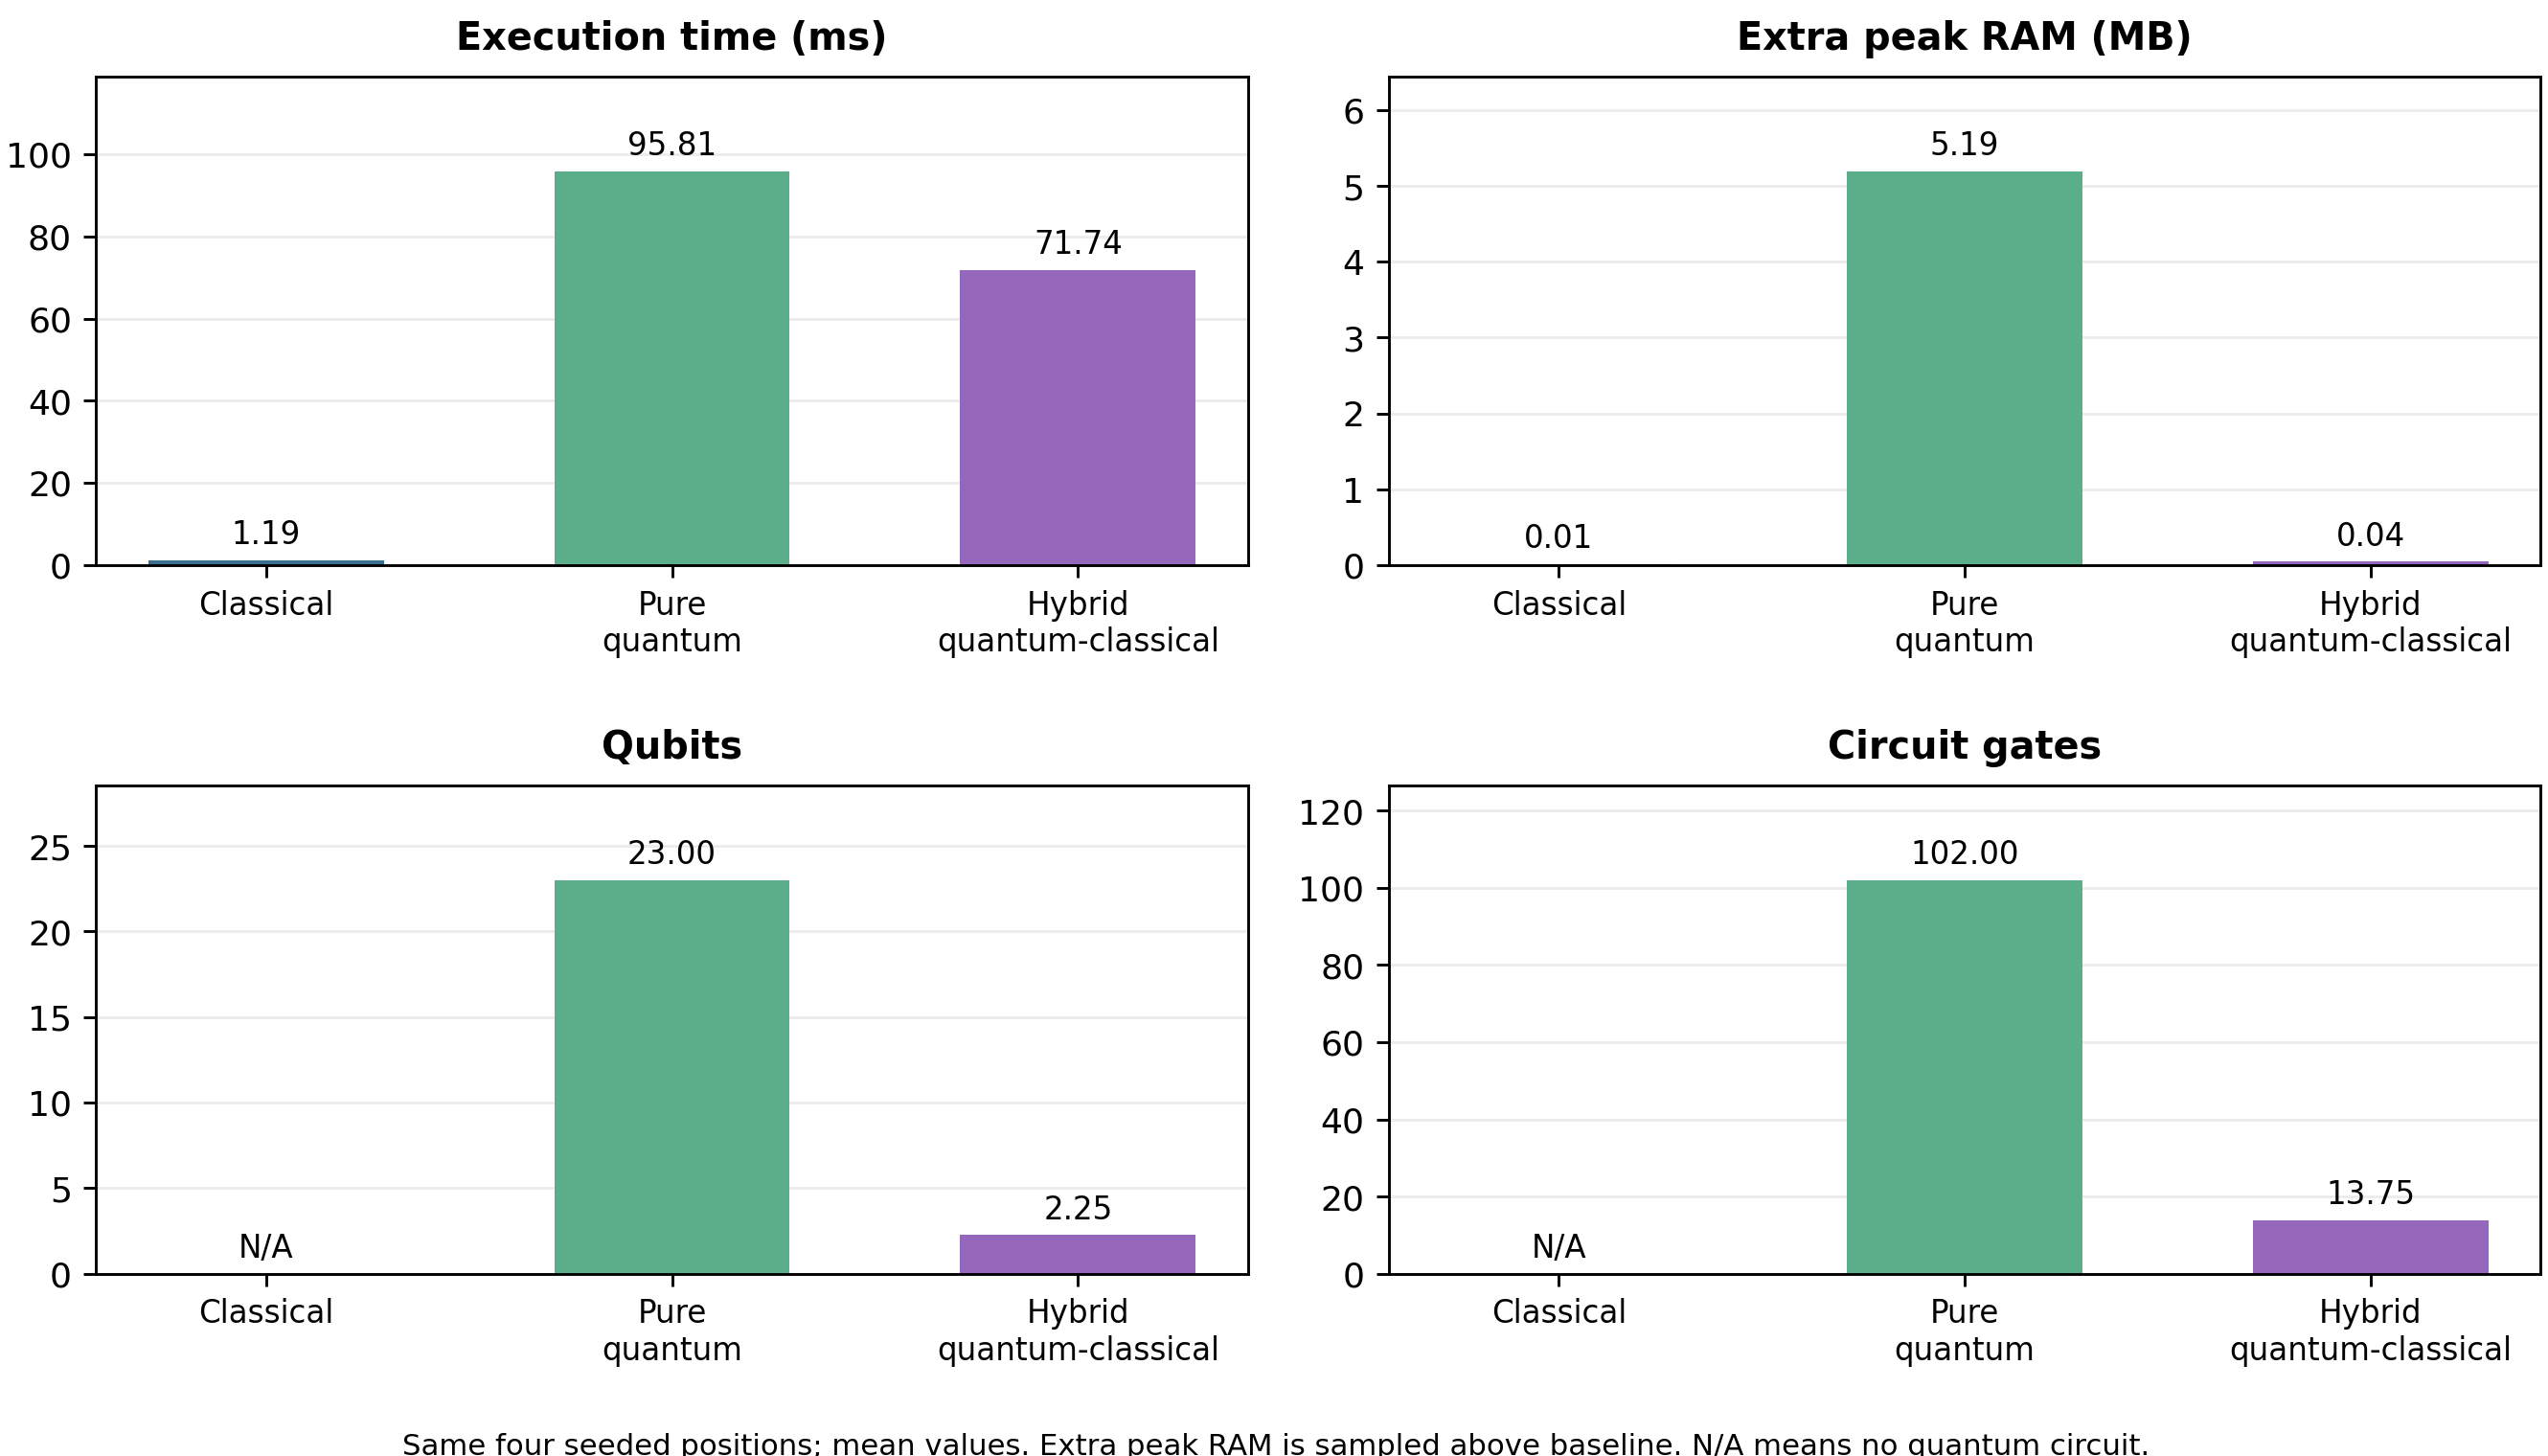
\includegraphics[width=0.98\textwidth]{results_3x3.png}
\caption{Measured time, additional peak memory, qubits, and gate counts. N/A denotes a classical run with no circuit.}
\label{fig:results}
\end{figure*}

\section{Conclusion and Outlook}
The project provides a transparent bridge between classical chess logic and quantum-circuit concepts. Its strongest implemented quantum-search example is the 8$\times$8 hybrid pipeline: legal moves and heuristic targets are prepared classically, then a Grover circuit amplifies selected indices. The 2$\times$2 and 3$\times$3 circuits help inspect gate-level encodings but remain prototypes. In the measured 3$\times$3 run, classical minimax had the smallest runtime and memory cost; the hybrid Grover circuit was structurally smaller than the pure-circuit demonstration but did not outperform the classical baseline.

Next work should define an injective encoding for every piece and empty square, implement and verify reversible legality and scoring oracles, and uncompute temporary data. The small-board transition should be checked against truth tables before adding complete board updates. Experiments should include a larger and broader position set, repeated runs with uncertainty estimates, equivalent end-to-end workloads, explicit oracle costs, and separate noise-on and hardware measurements. Move quality should be measured against a specified classical reference. Until those steps are complete, results should be described as simulator measurements of a hybrid prototype.

\appendices
\section{Circuit and Implementation Supporting Material}
The repository contains the implementation modules for move generation, minimax, heuristic scoring, Grover's oracle and diffuser, Aer execution, register encoding, and the small-board circuit builder. The complete system flow is summarized in Fig.~\ref{fig:architecture}. Fig.~\ref{fig:2x2} gives the detailed 2$\times$2 example, and Fig.~\ref{fig:circuit} shows the small-board register circuit. These figures document the prototype wiring. In particular, the coordinate/status circuit and Grover index circuit are separate: measurement of the former does not feed the latter.

\begin{figure*}[p]
\centering
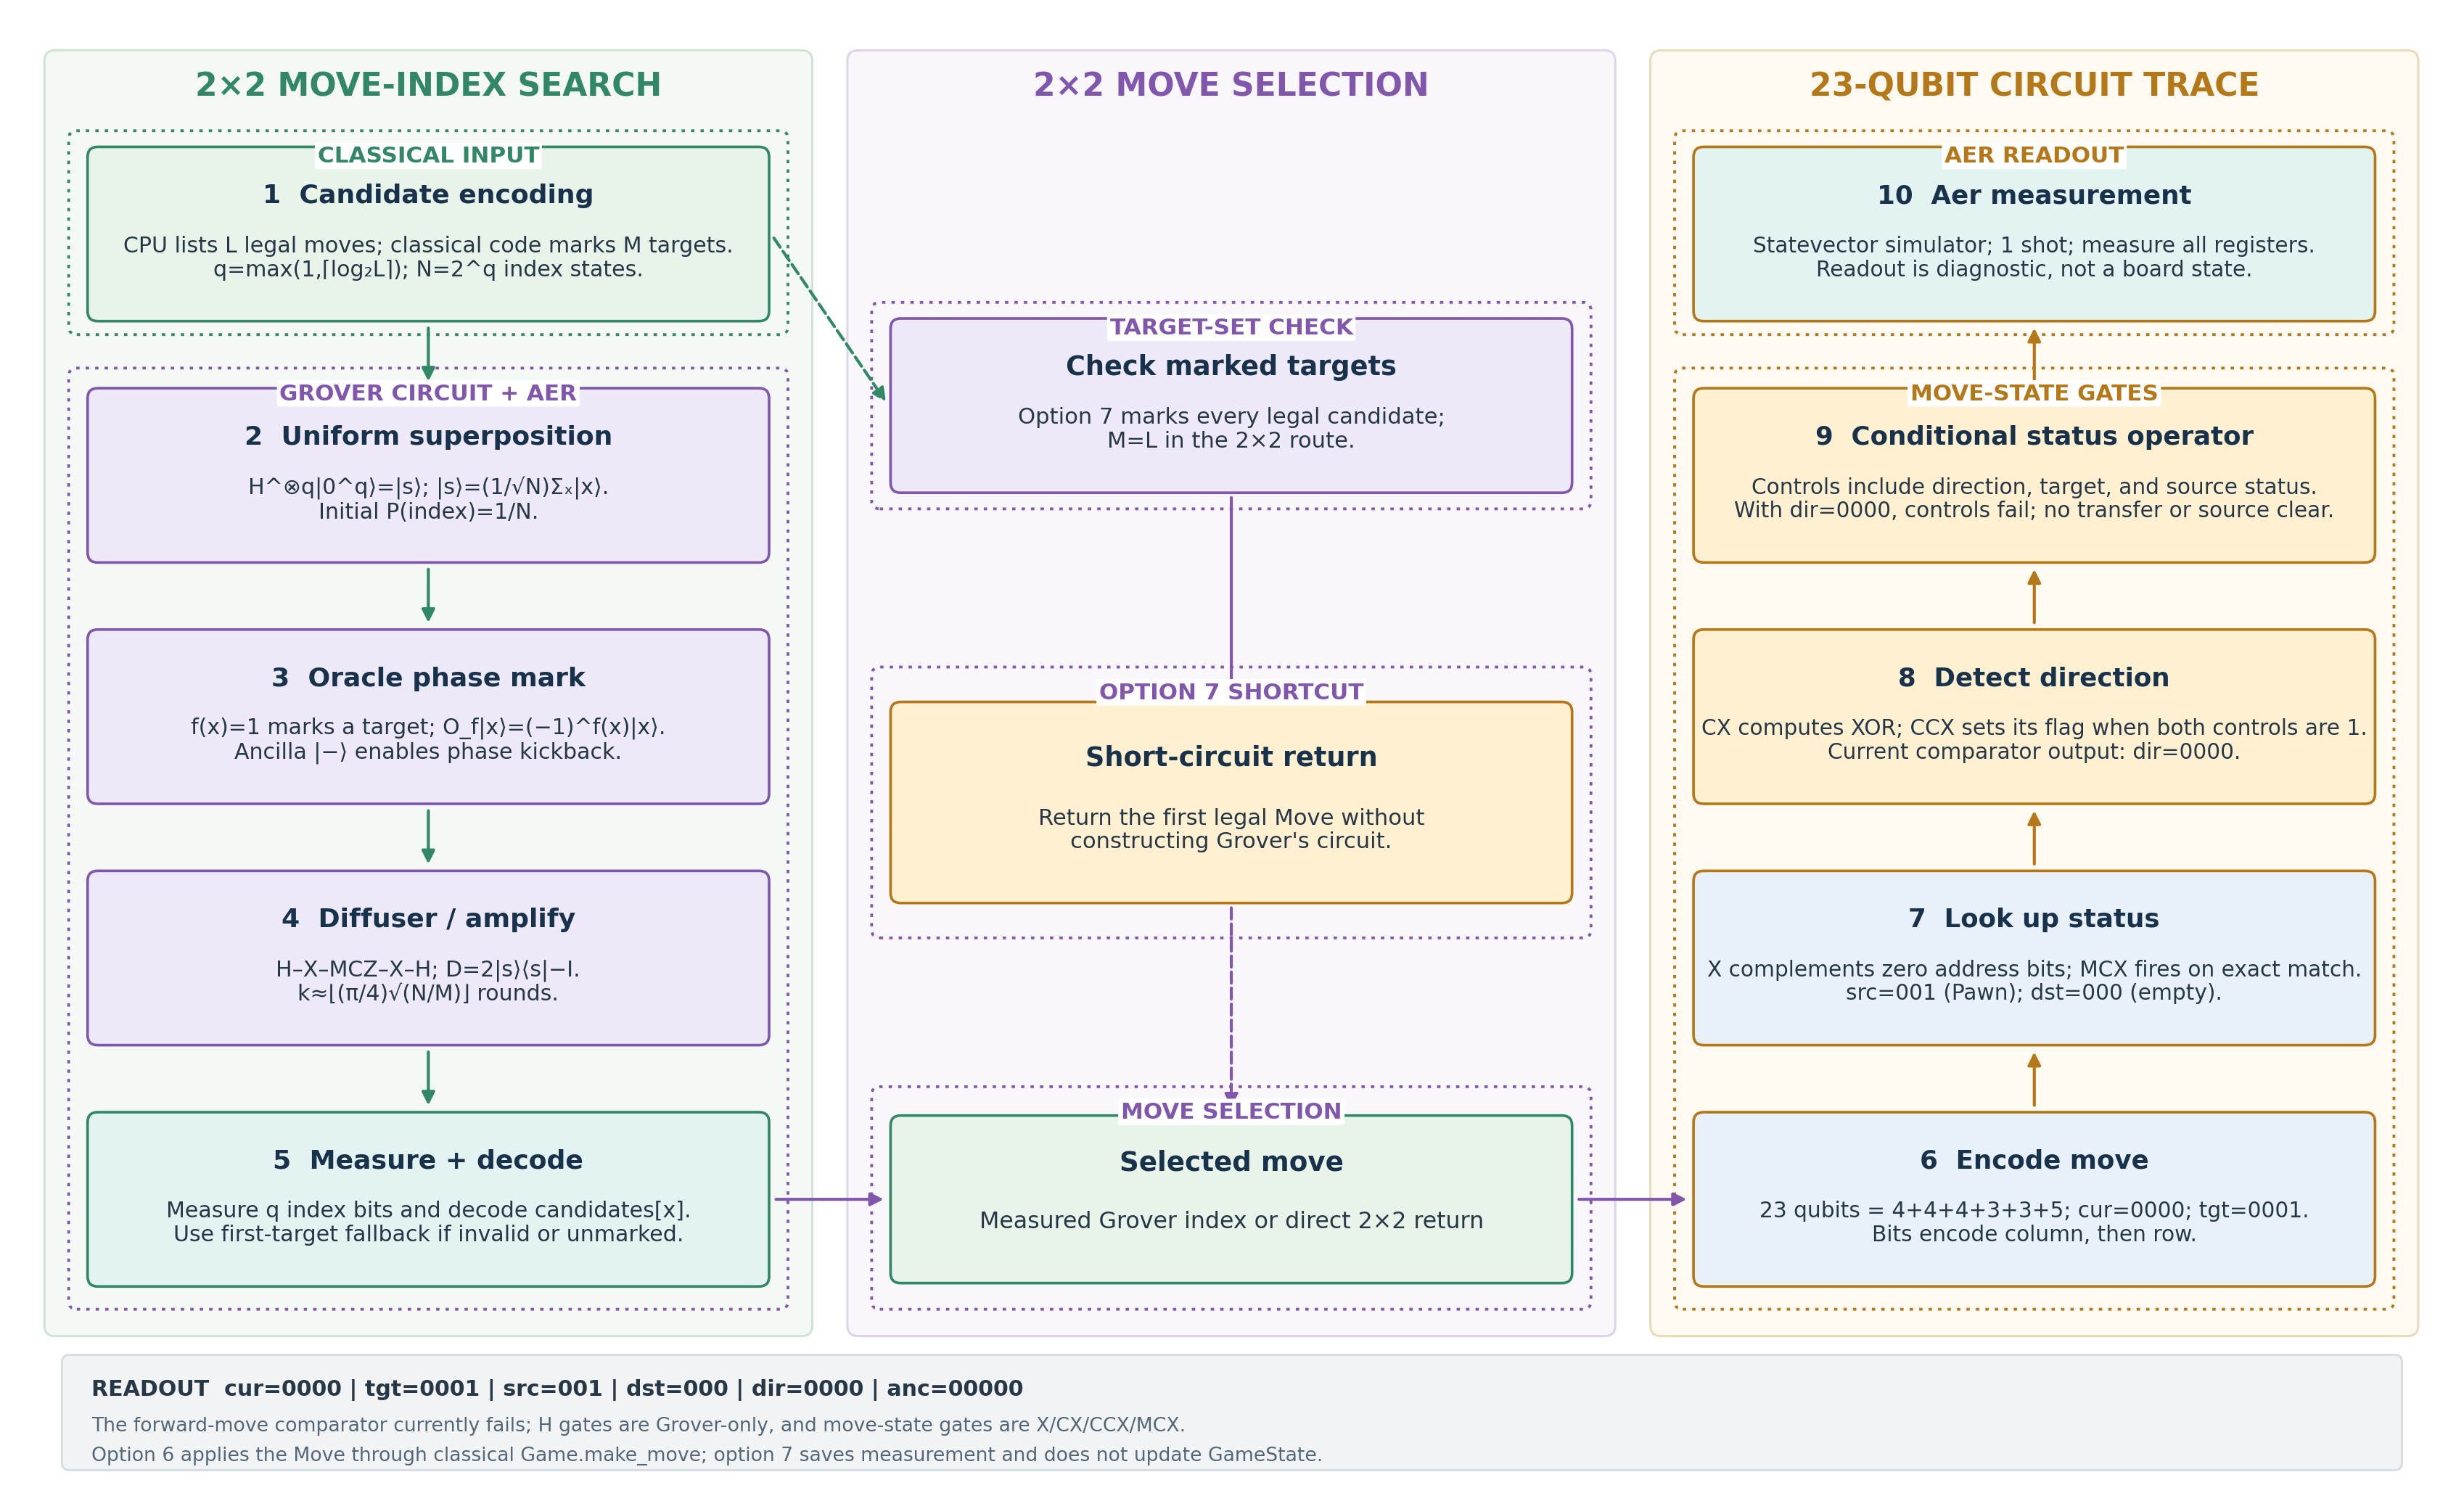
\includegraphics[width=0.98\textwidth]{12_2x2_grover_circuit_flow.png}
\caption{2$\times$2 move-index search and selected-move circuit flow. In the current one-candidate setup, the all-target shortcut returns the move without building Grover's circuit.}
\label{fig:2x2}
\end{figure*}

\begin{figure*}[p]
\centering
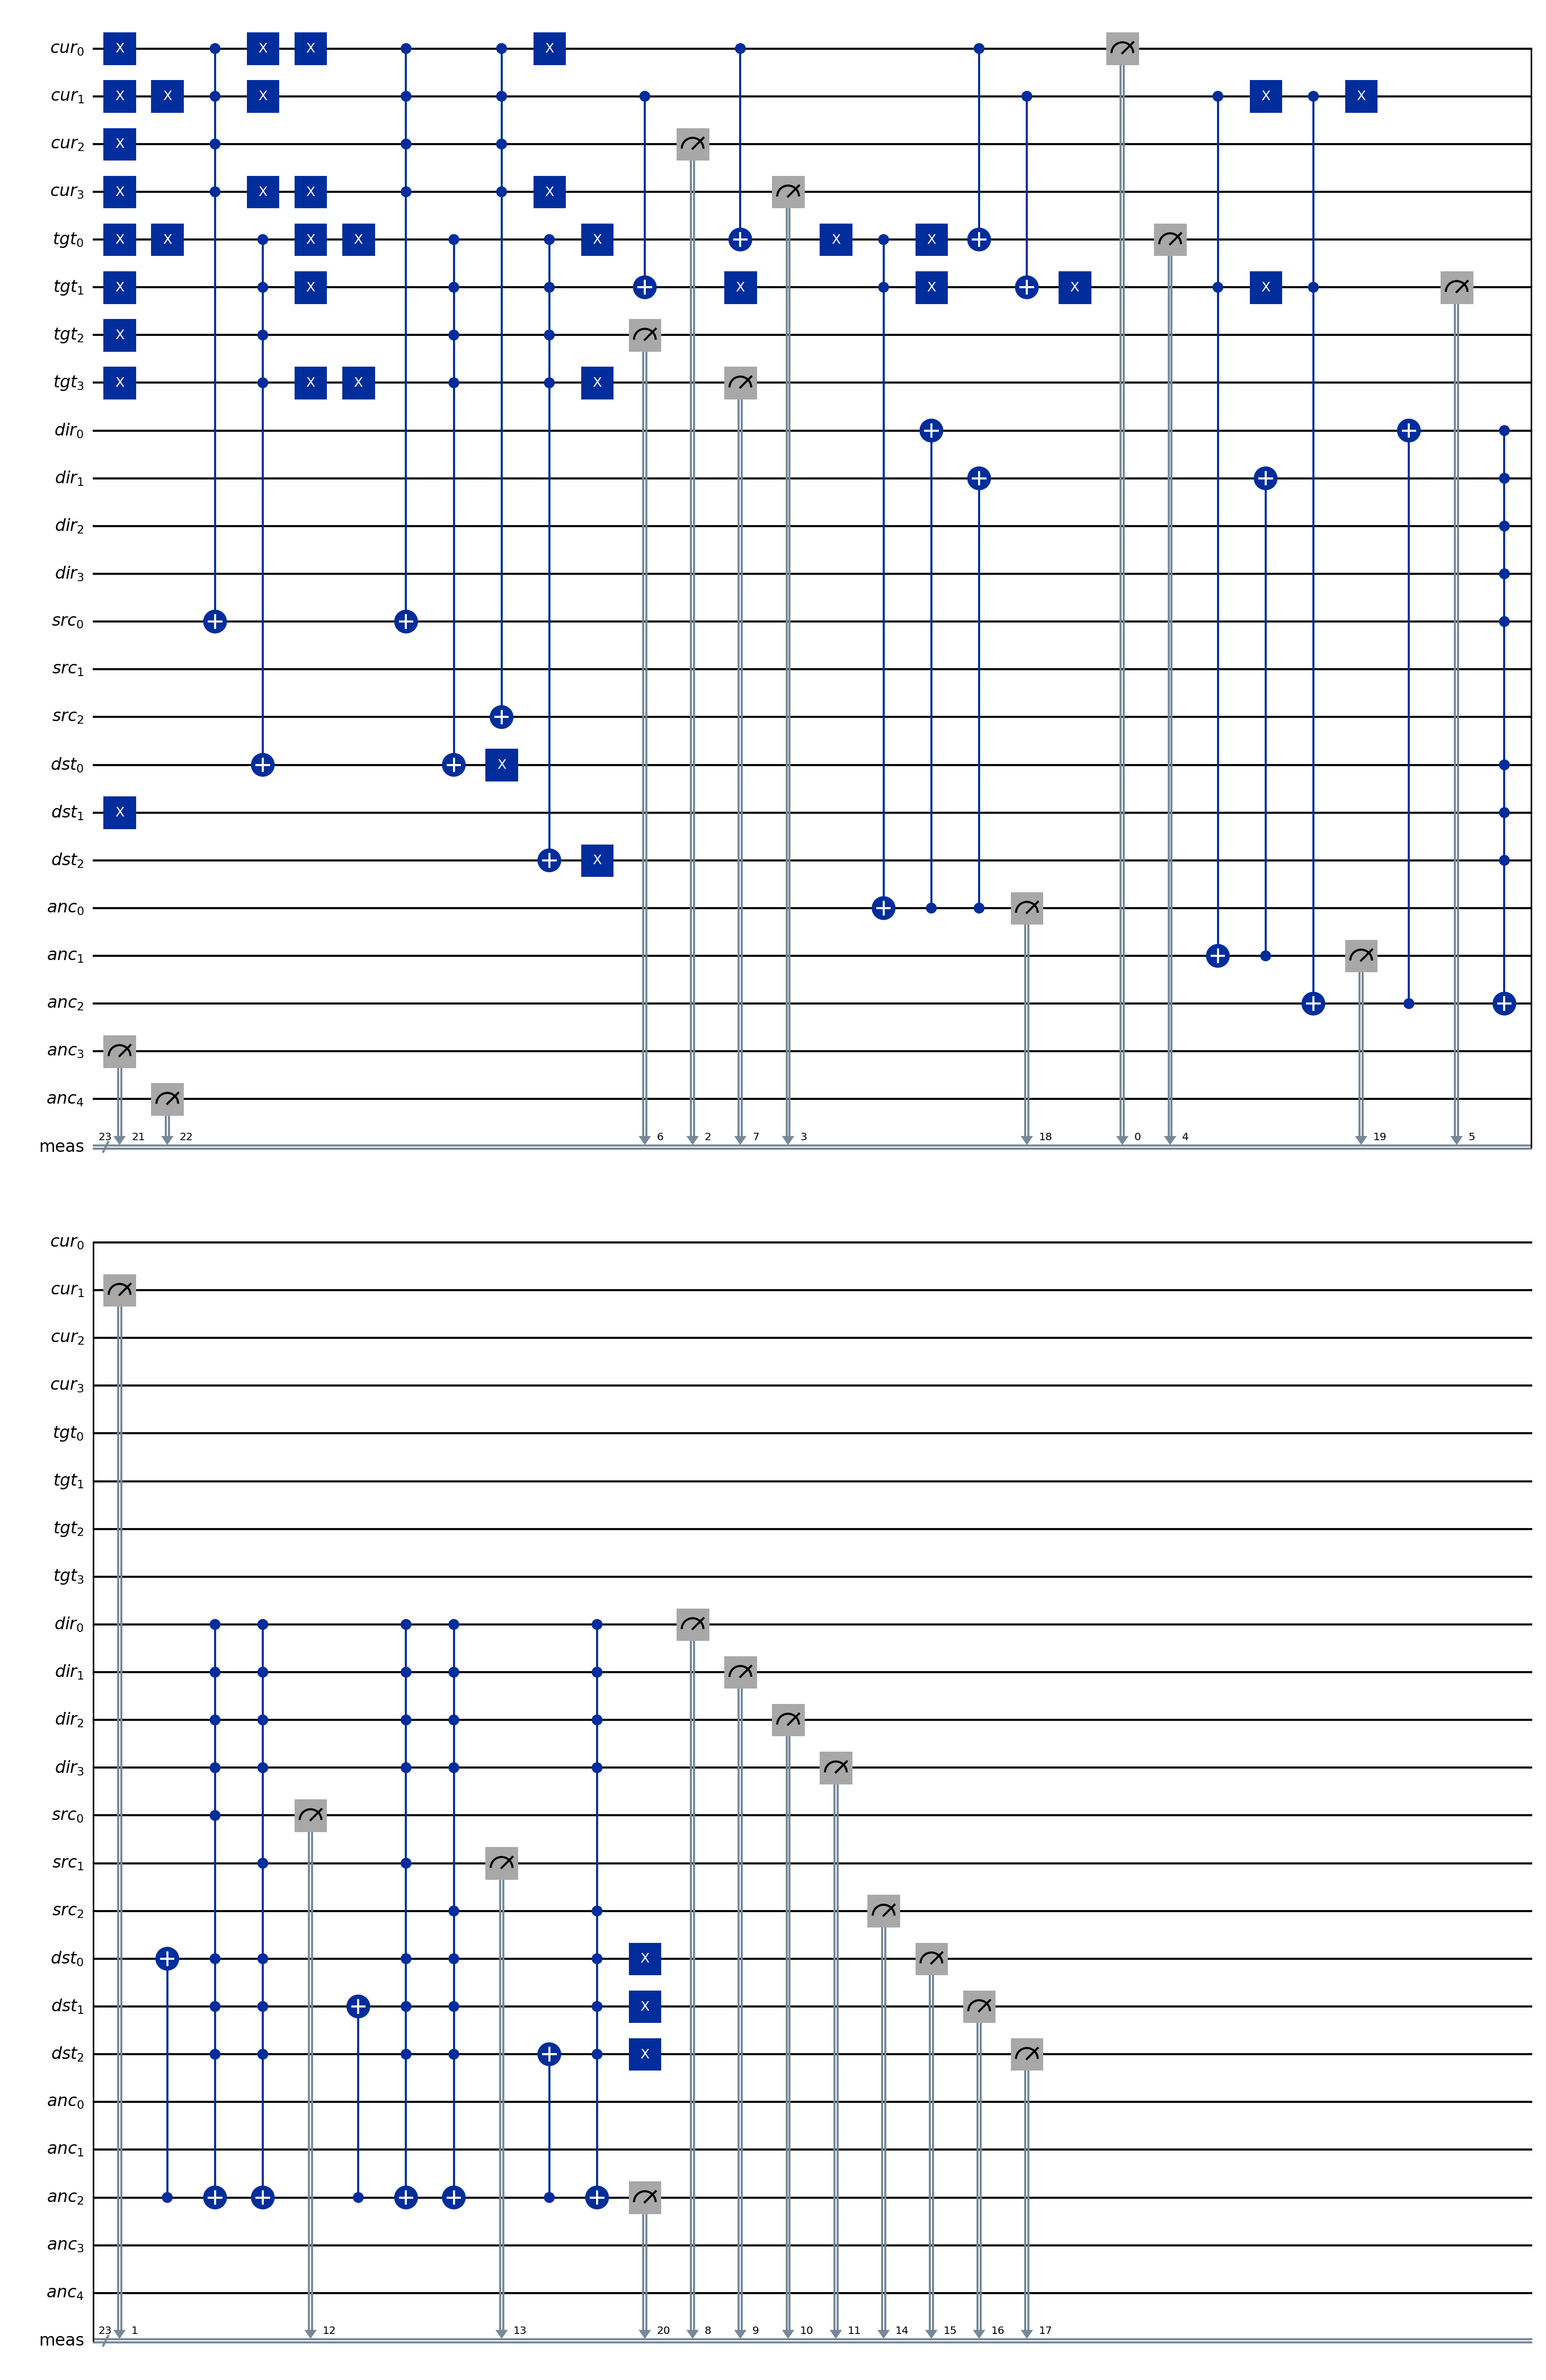
\includegraphics[height=0.78\textheight,keepaspectratio]{pure_quantum_3x3_circuit.png}
\caption{Small-board coordinate/status circuit diagram. The circuit is a prototype and its measurement is diagnostic.}
\label{fig:circuit}
\end{figure*}

\section{Reproducibility Notes}
The benchmark entry point is \texttt{evaluation/compare\_3x3\_systems.py}; summary and per-position measurements are under \texttt{evaluation/results/}. The evaluation uses seed 20261013, four positions, depth 3, 2048 hybrid shots, and one pure-circuit shot per position. The comparison script fixes the Aer CPU matrix-product-state simulator and disables noise. It excludes simulator initialization from timed selections. The report's exact result values are those stored in \texttt{evaluation/results/3x3\_comparison\_summary.csv}. The full project source and diagrams should accompany this paper when required by the course.

\subsection{Hybrid Move-Index Search Pseudocode}
The excerpt below summarizes the implementation boundary: candidates and target indices are computed classically, Grover amplifies the marked indices, and a classical decoder maps the measurement back to the candidate list.
\begin{verbatim}
legal = generate_legal_moves(state)
scores = [score_move(state, move) for move in legal]
targets = indices_with_maximum_score(scores)
if every candidate is marked: return legal[targets[0]]
n = max(1, ceil(log2(len(legal))))
prepare H^n index state and |-> flag
repeat phase_oracle(targets); diffuser()
index = measure_and_decode()
return legal[index] if valid target else legal[targets[0]]
\end{verbatim}
The corresponding source is in \texttt{ai/quantum\_search.py} and \texttt{quantum/grover.py}; the reversible oracle and diffuser are in \texttt{quantum/oracle.py} and \texttt{quantum/diffuser.py}.

\balance
\bibliographystyle{IEEEtran}
\bibliography{IEEE_Quantum_Chess_Project_Report}
\end{document}
